\documentclass[10pt,aspectratio=169]{beamer}

\usetheme{metropolis}
\usepackage[utf8]{inputenc}
\usepackage[T1]{fontenc}
\usepackage[english]{babel}
\usepackage{listings}
\usepackage{booktabs}
\usepackage{amsmath,amssymb}
\usepackage{tikz}
\usetikzlibrary{positioning,arrows.meta}

\definecolor{gfblue}{HTML}{1F4E79}
\definecolor{codebg}{HTML}{F4F4F2}
\definecolor{warn}{HTML}{B03A2E}
\definecolor{good}{HTML}{1E6B3A}
\definecolor{unitbg}{HTML}{FBF8EF}
\definecolor{textbg}{HTML}{F3FAF2}

\setbeamercolor{frametitle}{bg=gfblue}
\setbeamercolor{alerted text}{fg=warn}

\lstset{
  basicstyle=\ttfamily\scriptsize,
  backgroundcolor=\color{codebg},
  frame=none,
  columns=fullflexible,
  keepspaces=true,
  showstringspaces=false,
  breaklines=true,
  xleftmargin=2mm,
}

\newcommand{\bad}[1]{\textcolor{warn}{#1}}
\newcommand{\ok}[1]{\textcolor{good}{#1}}
\newcommand{\commit}[1]{\texttt{\footnotesize #1}}
\newcommand{\file}[1]{\texttt{#1}}
\tikzset{box/.style={draw, rounded corners, fill=#1, align=center, font=\small, minimum height=9mm, inner sep=4pt},
  box/.default=codebg}

\title{Informalizing Unit with Informath}
\subtitle{Gauss's lemma and gcd domains: Unit, Dedukti, English}
\author{Aarne Ranta, with Claude Code}
\date{November 2026}

\begin{document}

\maketitle

%----------------------------------------------------------------------
\begin{frame}{The task}

\small
\begin{itemize}
\item \textbf{Unit} (Thierry Coquand): a dependent type checker with segments
  (modules), records, universe levels, data types with \texttt{split}
\item The request: translate Unit to \textbf{Dedukti}, preserving
  type-correctness and the segment structure, so that \textbf{Informath} can
  read Unit developments as it reads Mathlib, Edukera, Godement
\item The test case: \file{unit/sag/gcddomain}, 23 files, 2414 lines
  \begin{itemize}
  \item Gauss's lemma, and ``if $A$ is a gcd domain, then so is $A[X]$''
  \item with an informal text by Thierry, \file{gcddomain.tex}: a
    \emph{level~C} proof in the sense of van Benthem Jutting, written
    file by file to test the claim that Unit's proof terms have the
    structure of a detailed informal proof
  \end{itemize}
\item So the informalization can be compared with a human text, proof by
  proof
\end{itemize}

\end{frame}

%----------------------------------------------------------------------
\begin{frame}{The pipeline}

\centering
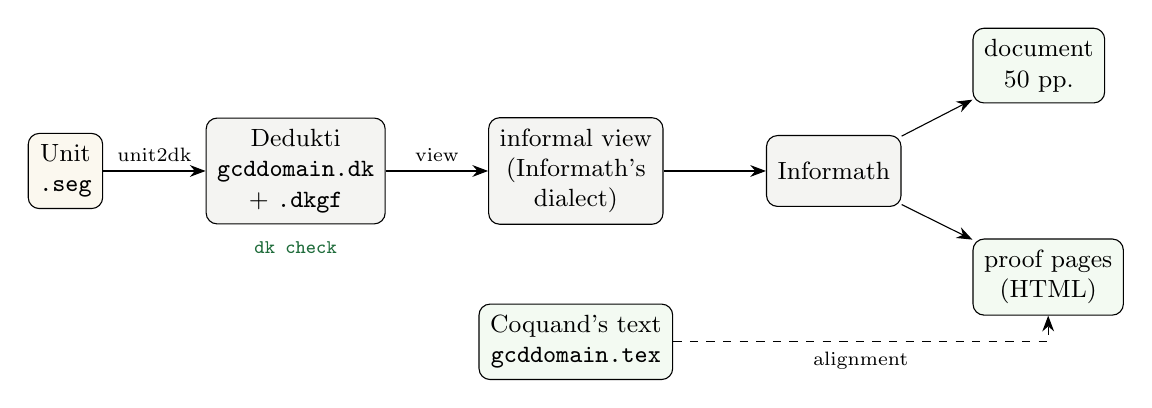
\begin{tikzpicture}[>={Stealth[length=2mm]}, node distance=6mm and 13mm]
\node[box=unitbg] (unit) {Unit\\\file{.seg}};
\node[box, right=of unit] (dk) {Dedukti\\\file{gcddomain.dk}\\+ \file{.dkgf}};
\node[box, right=of dk] (view) {informal view\\(Informath's\\dialect)};
\node[box, right=of view] (inf) {Informath};
\node[box=textbg, above right=4mm and 9mm of inf] (doc) {document\\50 pp.};
\node[box=textbg, below right=4mm and 9mm of inf] (proofs) {proof pages\\(HTML)};
\node[box=textbg, below=10mm of view] (orig) {Coquand's text\\\file{gcddomain.tex}};
\draw[->] (unit) -- node[above, font=\scriptsize]{unit2dk} (dk);
\draw[->] (dk) -- node[above, font=\scriptsize]{view} (view);
\draw[->] (view) -- (inf);
\draw[->] (inf) -- (doc);
\draw[->] (inf) -- (proofs);
\draw[->, dashed] (orig) -| node[below, near start, font=\scriptsize]{alignment} (proofs);
\node[below=1mm of dk, font=\scriptsize, text=good] {\texttt{dk check}};
\end{tikzpicture}

\vspace{4mm}
\begin{itemize}\small
\item \textbf{unit2dk} (Haskell): uses Unit's own checker as a library and
  Informath's Dedukti syntax; reads Unit's values back as typed Dedukti terms
\item \textbf{Python scripts}: \file{informal\_view.py}, \file{informal\_doc.py},
  \file{proof\_sample.py}, \file{align.py}
\end{itemize}

\end{frame}

%----------------------------------------------------------------------
\section{From Unit to Dedukti}

\begin{frame}[fragile]{The encoding (\file{prelude.dk})}

\begin{columns}[T]
\begin{column}{0.48\textwidth}
\small
\begin{itemize}
\item \textbf{Levels}: \texttt{Lvl}, \texttt{lz}, \texttt{ls}, and
  \texttt{defac lmax} with absorption rules
\item \textbf{Universes} \`a la Tarski: codes \texttt{U l}, decoding
  \texttt{El l}, cumulativity by \texttt{lift}
\item \textbf{$\Pi$, $\Sigma$, Id} as codes; \texttt{J} computing on
  \texttt{refl}
\item \textbf{Data types}: constants; \texttt{split} as rewrite rules
\item \textbf{Segments}: lambda-lifted; \texttt{\#STRUCTURE} lines in the
  \file{.dkgf}
\end{itemize}
\end{column}
\begin{column}{0.5\textwidth}
\begin{lstlisting}
defac lmax [Lvl].
[l, r] lmax l (lmax (ls l) r) --> lmax (ls l) r.
[l, r] lmax l (ls (lmax l r)) --> ls (lmax l r).

U : Lvl -> Type.
def El : l : Lvl -> U l -> Type.
def pi : l1 : Lvl -> l2 : Lvl -> a : U l1 ->
  (El l1 a -> U l2) -> U (lmax l1 l2).
[l1, l2, a, b] El _ (pi l1 l2 a b)
  --> x : El l1 a -> El l2 (b x).
\end{lstlisting}
\end{column}
\end{columns}

\end{frame}

%----------------------------------------------------------------------
\begin{frame}[fragile]{Records: the typed encoding}

\begin{columns}[T]
\begin{column}{0.42\textwidth}
\begin{lstlisting}[backgroundcolor=\color{unitbg}]
record CRing {
  R : U a ;
  z : R ; o : R ;
  add : R -> R -> R ;
  mul : R -> R -> R ;
  ...
  mulO (x : R) : Id R (mul x o) x ;
  ...
} ;
module RL (Rg : CRing) { open Rg ; ... }
\end{lstlisting}
\end{column}
\begin{column}{0.56\textwidth}
\begin{lstlisting}
CRing    : a : Lvl -> U (ls a).
CRing.mk : a : Lvl -> R : U a -> z : El a R
  -> ... -> El (ls a) (CRing a).
def CRing.mul : a : Lvl -> t : El (ls a) (CRing a)
  -> El a (CRing.R a t) -> ... .
[a, R, z, ...] CRing.mul a (CRing.mk a R z ...)
  --> mul.
\end{lstlisting}
\end{column}
\end{columns}

\vspace{2mm}
\small
\begin{itemize}
\item a type, a constructor, a \emph{selector} per field with its rule;
  derived members take the element; nominal, no $\eta$, as in Unit
\item \file{.dkgf}: \texttt{\#RECORD CRing CRing.mk CRing.R ...}, for
  Informath to read the constructor as a structure definition
\item \textbf{Fixed fields}: \texttt{isEquiv A B f = IsEquiv[A, B, f]} is
  a record of its own, \texttt{IsEquiv[A,B,f]}, with a coercion
  \texttt{.up} to \texttt{IsEquiv}; the variants used are found by
  translating again until none is missing
\end{itemize}

\end{frame}

%----------------------------------------------------------------------
\begin{frame}{Results on \file{sag/gcddomain}}

\centering
\begin{tabular}{lrr}
\toprule
 & first version & now \\
\midrule
declarations translated in full & 111 & \ok{612} \\
as axioms & 55 & 0 \\
left out & 444 & 0 \\
\midrule
accepted by \texttt{dk check} & --- & \ok{689 declarations, 220 rule sets} \\
demoted & --- & 1 \\
\bottomrule
\end{tabular}

\vspace{5mm}
\begin{itemize}\small
\item The one demoted: \texttt{FunExtUA.FE.totC}, which needs $\eta$ for
  $\Sigma$ on neutral terms: Dedukti's matching does not see
  \texttt{pair (x => fst p x) (x => snd p x)} as \texttt{p}
\item Translation time: 0.1\,s (twice, for the variants of records)
\end{itemize}

\end{frame}

%----------------------------------------------------------------------
\begin{frame}{Found and fixed on the way}

\small
\begin{itemize}
\item \textbf{Unit changed under us}: indexed inductive families arrived
  (5 Nov); the translator adapted, and a misreading of mine (taking every
  parametrized data type for a family) cost 500 declarations until fixed
\item \textbf{Levels}: \texttt{lmax} is AC, but rules like
  \texttt{lmax l (ls l) --> ls l} match only a whole join; rules with a
  variable for the rest, and absorption under a successor, were needed
\item \textbf{Parameter types at instances}: reading a type back and
  evaluating it again turned \texttt{PolyR.P} into a rigid constant;
  the type is now evaluated from its syntax
\item \textbf{Dedukti's grammar}: \texttt{(f : A -> B)} is the type
  \texttt{(f : A) -> B}, in the official grammar too; a field of function
  type is written \texttt{(f : (A -> B))}
\item \textbf{Informath}: now parses \texttt{defac} / \texttt{defacu}
\end{itemize}

\end{frame}

%----------------------------------------------------------------------
\section{From Dedukti to English}

\begin{frame}{The informal view}

\small
unit2dk's Dedukti is checkable, not readable. \file{informal\_view.py}
rewrites it into Informath's dialect (\texttt{Set}, \texttt{Elem},
\texttt{Proof}, \texttt{forall}, \texttt{exists}, \ldots):

\begin{itemize}
\item \textbf{dropped}: levels, lifts, and the foundations' parameters
  (\texttt{univ}, \texttt{images}, \texttt{surjections})
\item \textbf{\texttt{El} of a code}: a function type, an equation
  \texttt{Proof (Id A x y)}, a proposition \texttt{Proof P}, or
  \texttt{Elem A}
\item \textbf{propositions} are recognized: identity types,
  \texttt{Empty}, \texttt{Not}, sums of propositions (decisions), $\Pi$ and
  $\Sigma$ of propositions (\emph{for all}, \emph{there exists}), and
  constants defined as such (\texttt{Div}, \texttt{GcdOf})
\item \textbf{records} are structures; their selectors become notation;
  binary operations are \texttt{Oper} fields named by their symbols
\item \textbf{names} shortened: \texttt{div\_trans},
  \texttt{Gcd\_gcd}
\end{itemize}

\file{gcddomain-view.dkgf}: about 50 symbol table entries in the
notation of Thierry's text: $a\mid b$, $\mathrm{c}(f)$, $p_k$,
$a + Xp$, $A[X]$; one new word in \file{Mathlib.gf}: \emph{gcd domain}

\end{frame}

%----------------------------------------------------------------------
\begin{frame}{Readings}

\small
\textbf{Structure.} A commutative ring is an algebraic structure, where
$R$ is a set, $z$ is an element of $R$, \ldots, $+$ is a binary operation
on $R$, \ldots, for all elements $x$, $y$ and $w$ of $R$,
$x + (y + w) = (x + y) + w$, \ldots

\medskip
\textbf{Definition.} Let $A$ be a commutative ring. Let $a$ and $b$ be
elements of $R$. Then $a$ divides $b$, if there exists an element $q$ of
$R$ such that $b = aq$.

\medskip
\textbf{Div\_trans.} Let $a$, $b$ and $c$ be elements of $R$ such that $a$
divides $b$ and $b$ divides $c$. Then $a$ divides $c$.

\medskip
\textbf{Gauss.} Let $p$ and $q$ be elements of $\mathcal{P}$ such that the
function that maps $k$ to $p_k$ is primitive. Let $d$ be an element of $R$
such that $d$ is a common divisor of the coefficients of $pq$. Let $i$ be
a natural number. Then $d$ divides $q_i$.

\medskip
\textbf{The main theorem.} Let $A$ be a commutative ring. Let $G$ be a gcd
domain on $A$. Then \texttt{Over\_domain} applied to $A$ and $G$ is a gcd
domain on $A[X]$.

\end{frame}

%----------------------------------------------------------------------
\begin{frame}{The document}

\small
\file{informal\_doc.py}: one section per segment, its parameters said
once, as an informal text does:

\begin{block}{GcdDomain.Domain}
\emph{In this section:} Let $A$ be a commutative ring. Assume that $R$ is
a set. Assume that for all elements $x$ of $R$, $x = 0$ or $x$ is not equal
to $0$. Assume that for all $x$ and $y$ \ldots

\textbf{Sub\_zero.} Let $a$ and $b$ be elements of $R$ such that
$a + -b = 0$. Then $a = b$.
\end{block}

\begin{itemize}
\item 635 of 636 declarations read, 57 sections, 50 pages, LaTeX without
  errors
\item the section's parameters come from the \texttt{\#STRUCTURE} lines
  of unit2dk's \file{.dkgf}; the context sentence is Informath's reading
  of them as hypotheses
\end{itemize}

\end{frame}

%----------------------------------------------------------------------
\section{Proofs}

\begin{frame}{Proof texts}

\footnotesize
Informath's \texttt{-proof-text} reads a proof term as numbered lines,
each justified by the rule it applies. For Unit's proofs, the view writes
the rules (types in \file{unit-nd.dk}):

\begin{itemize}
\item a pair proving a $\Sigma$ of a proposition: \texttt{existsI}; its
  projections \texttt{fst}, \texttt{snd}
\item \texttt{J} at a motive not using the path (the steps of
  \texttt{calc}): \texttt{trans}, or \texttt{transport}
\item a hypothesis applied to arguments: \texttt{forallE}, \texttt{ifE},
  unfolding defined propositions (\texttt{Rec N}, \texttt{Common d f})
\item a $\lambda$ proving \emph{for all} or \emph{if}: \texttt{forallI},
  \texttt{ifI}
\end{itemize}

\textbf{div-trans}, with \texttt{-force-symbolic}:

\begin{tabular}{rll}
1. & Assume that $a\mid b$. & \\
2. & Assume that $b\mid c$. & \\
3. & $c = b\,\pi_1(k)$. & \texttt{snd} 2 \\
\ldots \\
9. & $c = a(\pi_1(h)\,\pi_1(k))$. & \texttt{trans} 3, 8 \\
10. & There exists an element $q$ of $R$, such that $c = aq$. & \texttt{existsI} 9 \\
\end{tabular}

\end{frame}

%----------------------------------------------------------------------
\begin{frame}[fragile]{The proof pages}

\footnotesize
\file{proof\_sample.py}: for each proof, a table of its steps,
numbered as the proof text numbers its lines (the hypotheses first, then
each step after its premisses; checked against the lines' rules):

\vspace{1mm}
\scriptsize
\begin{tabular}{rp{0.30\textwidth}lp{0.32\textwidth}}
\toprule
\# & Informath & by & Unit \\
\midrule
3 & $a\mid ca$. & \texttt{div\_factor\_left} & \texttt{\ \ div-factor-left a c} \\
4 & $bc = cb$. & \texttt{mulC} & \texttt{\ \ mulC b c} \\
5 & $a\mid cb$. & \texttt{div\_eq\_right} 4, 2 & \texttt{\ \ div-eq-right a (mul b c) (mul c b) 4 2} \\
6 & $a\mid c\gcd(a,b)$. & \texttt{lemma\_M} 3, 5 & \texttt{\ \ \ \ lemma-M c a b a 3 5} \\
\ldots \\
10 & By div\_trans, $a\mid c$. & \texttt{div\_trans} 6, 9 & \texttt{div-trans a (mul c (gcd a b)) c 6 9} \\
\bottomrule
\end{tabular}

\vspace{1mm}
\footnotesize
\begin{itemize}
\item a step is its rule applied to its other arguments, the numbers of
  its premisses (links) in place of their proofs, indented by depth
\item the Unit column omits what Unit's source omits (implicit arguments,
  module parameters): it reproduces the source of \texttt{euclid}
\item a Dedukti column, hidden behind a toggle; the Unit source and the
  whole proof term above the table
\end{itemize}

\end{frame}

%----------------------------------------------------------------------
\begin{frame}{Aligning Thierry's text with the steps}

\footnotesize
\file{align.py}, automatic:

\begin{enumerate}
\item \textbf{find the text} by \texttt{\textbackslash nm\{name\}}: a lemma titled with it,
  an item of a lemma's list and the paragraph ``(k)'' of its proof, or an
  item of a module's proof (\texttt{Tail.eq})
\item \textbf{cut it} at its formulas; chains $c = bk = (ah)k$ at their
  relations
\item \textbf{parse the formulas} ($\mid$, $=$, products, sums, $\gcd$,
  $\mathrm{c}(p)$, $q_{i+1}$, $a+Xp$) and normalize the steps' conclusions
  the same way
\item \textbf{link} a fragment to the steps whose conclusions it states:
  equations either way round; $\pi_1(h)$ as $h$; a letter that is not a
  variable of the theorem (a quotient $q$) matching any term; polynomial
  identities by their coefficients; local definitions ($t=\gcd(d,a_0)$)
  by their values; claims in words (``is a common divisor of'', ``is
  primitive''); names of lemmas used
\end{enumerate}

\begin{block}{div-trans, (4)}
\colorbox{yellow!30}{If $b = ah$}$_{[4]}$
\colorbox{yellow!30}{and $c = bk$}$_{[3]}$
then \colorbox{yellow!30}{$c = bk$}$_{[3]}$
\colorbox{yellow!30}{$= (ah)k$}$_{[5]}$
\colorbox{yellow!30}{$= a(hk)$}$_{[6\text{--}9]}$,
\colorbox{yellow!30}{so the quotient is $hk$}$_{[10]}$.
\end{block}

\end{frame}

%----------------------------------------------------------------------
\begin{frame}{Alignment results}

\centering
\small
\begin{tabular}{p{0.36\textwidth}ccc}
\toprule
sample & proofs & texts aligned & fragments linked \\
& & with the steps & \\
\midrule
divisibility: div-refl, div-of-zero, div-trans, euclid & 4 & 4 & as by hand, but 1 \\
Gauss's lemma: Tail, PrimStep.One, PrimStep & 11 & 11 & 23 of 28 \\
\bottomrule
\end{tabular}

\vspace{5mm}
\begin{itemize}\small
\item the unlinked fragments: words without formulas, ``by the claim
  for $a$, $p$, $g$'', ``apply $\mathrm{Rec}(N)$''
\item the hand-made alignment of the first sample is kept
  (\file{proof-sample.json}) for comparison
\item the text's proof of Gauss's lemma is a list of items, one per
  member of a Unit module: \emph{the proof terms do have the structure of
  the informal proof}, and the members are its steps
\end{itemize}

\end{frame}

%----------------------------------------------------------------------
\begin{frame}{Changes in Informath}

\small
\begin{itemize}
\item \texttt{defac} and \texttt{defacu} in the Dedukti grammar, read as
  declarations of binary operations \hfill\commit{b2f9f3c}
\item \texttt{gcd\_domain\_Noun} in \file{Mathlib.gf}, five languages
  \hfill\commit{0a59340}
\item \texttt{-to-latex-doc} escapes underscores in labels such as
  \texttt{div\_trans} \hfill\commit{41b41d7}
\item \texttt{\#EXCLUDE} also leaves out the rewrite rules of the excluded
  constants \hfill\commit{e043d27}
\end{itemize}

\textbf{Issues found, worked around in the view}:
\begin{itemize}
\item symbol table entries for names in \texttt{\{|...|\}} are never used
  (\texttt{lookupConstant})
\item a LaTeX macro of a constant used with fewer arguments than its
  notation breaks the output (the view $\eta$-expands)
\item Swedish \emph{var} for \emph{where} in structure definitions;
  \texttt{AdjKind} and \texttt{DepNoun} only in English and French
\end{itemize}

\end{frame}

%----------------------------------------------------------------------
\begin{frame}{What remains}

\small
\begin{itemize}
\item \textbf{Translation}: indexed inductive families (none in
  gcddomain); $\Sigma$-$\eta$ on neutral terms; Unit's \texttt{core}
  (100\,MB of output when local definitions are unfolded)
\item \textbf{Readings}: witnesses as $\pi_1(h)$ where a text says ``let
  $q$ be such that $b = aq$'' (an elimination of \emph{exists});
  definitions by \texttt{split} (\texttt{One.coeffs}) have rules, not
  proof terms
\item \textbf{Alignment}: the formula parser and the verbal claims are
  those of this text; a larger sample, and other texts, will show how far
  it carries
\item \textbf{The comparison itself}: Thierry's claim that the proof
  terms have the structure of the informal proof can now be inspected
  step by step, on pages that show both
\end{itemize}

\vspace{3mm}
\centering
\small Repository: \texttt{github.com/aarneranta/unit-informath}

\end{frame}

\end{document}
